In this section we describe the primary data collection, processing and storage resources available to the collaboration. 

\subsection{Data Acquisition Racks at HFIR}

\subsection{LC Resources at LLNL}
The Livermore Computing (LC) system includes a wide array of cluster computing and storage resources~\cite{lc}. Three primary LC systems will be used by PROSPECT:
\begin{itemize}
\item \textbf{HPSS}

The High Performance Storage System (HPSS)~\cite{HPSS} archival storage is comprised of server machines, RAID disk caches, magnetic tape libraries, and jumbo frame GigE network interconnections (Fig.~\ref{fig:HPSS}). 
It is designed to provide "virtually unlimited" tape archive storage in the petabyte range. Both capacity and performance are continually increasing to keep up with the ever increasing user demand.
The archive is never purged, but it is also not backed up.
Each individual user receives an annual storage quota of more than $100$~TB, i.e. can store new data of this volume per year. Access to group accounts and larger quotas can be requested as required.

\item \textbf{\texttt{oslic}}

A special purpose computing cluster, which has been optimized for high-speed data movement to HPSS storage. Detector data is transferred from HFIR to archival storage via \texttt{oslic}.

\item \textbf{\texttt{borax}}

The \texttt{borax} computer cluster comprises 1728 2.1~GHZ Intel Xeon EP CPUs~\cite{borax}. There are 48 nodes, with 36 CPUs and 128 GB RAM on each node. It operates at a peak performance of 58 TFLOPS. A project allocation is in place for PROSPECT. 

\end{itemize}

\begin{figure}
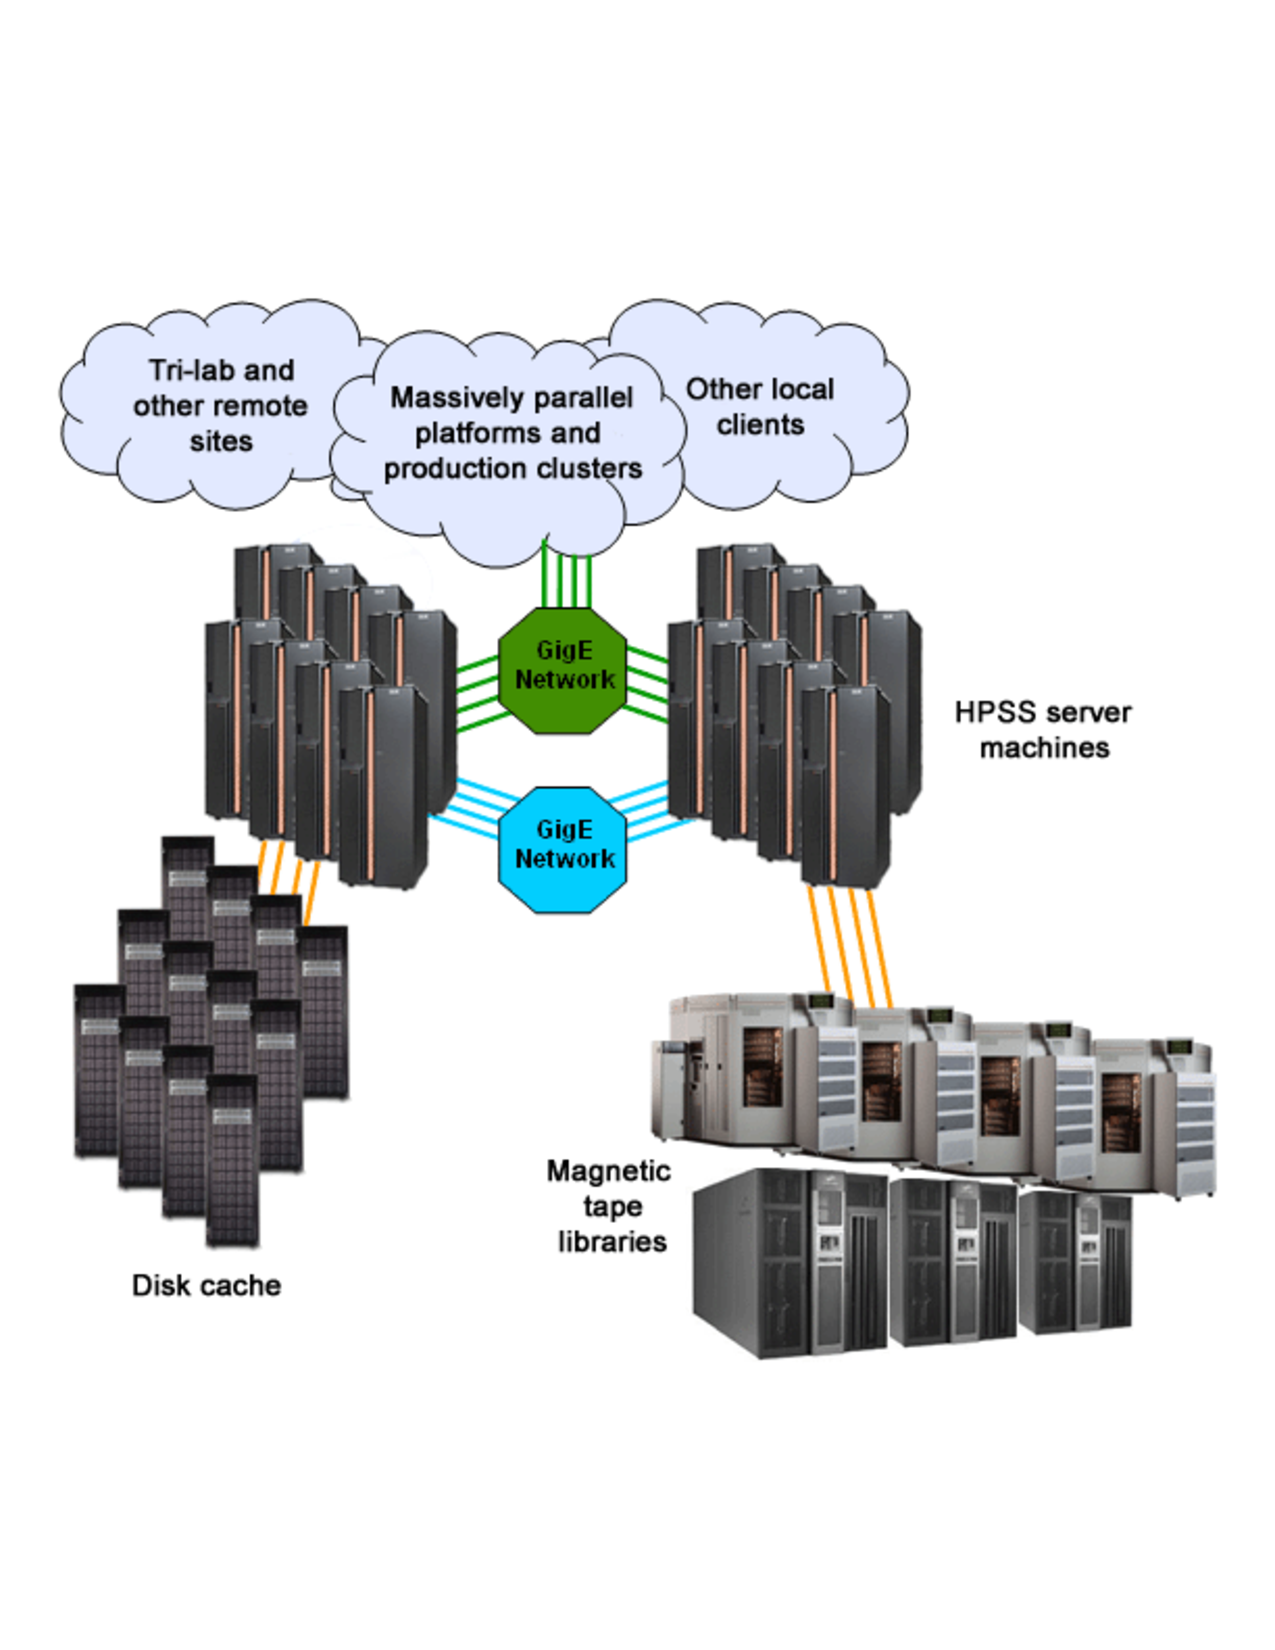
\includegraphics[width=0.50\textwidth]{figures/hpssDiagram.pdf}
\caption{Schematic of the LC HPSS storage archive.} \label{fig:HPSS}
\end{figure}

The resources described here are available at no cost to any PROSPECT collaborator.  


\subsection{Resources at ORNL}
The ORNL Physics Division hosts a computing cluster for data storage and analysis, composed of a 500~TB file store and 55 nodes of heterogeneous computers.  The cluster has 636 cores of INTEL and AMD processors, running RHEL 7.  The cluster is shared with COHERENT, MAJORANA, and other Physics Division research.  About 100TB can be made available for PROSPECT use, if required.  Additional disk storage can be added at cost.

The filestore, phybfs1.phy.ornl.gov and the head node, hcdata.phy.ornl.gov are connected to the laboratory network via 10Gbit Ethernet.  The newer compute nodes are, as well.  The older nodes are connected by 1Gb/s links.  The filestore is a Globus Interconnect endpoint, for data transfer within the laboratory and to the Internet.  Simpler file protocols, bbcp, rsync and sftp, are also available. 

\subsection{Resources at Yale University}
Yale University provides substantial computational resources utilized by the PROSPECT collaboration.
These include locally maintained systems at Wright Laboratory and university-maintained High Performance Computing and large-scale data storage.
\subsubsection{Yale Wright Laboratory}
The Yale Wright Laboratory hosts two computing systems for data storage and analysis. 
These systems (wright.physics.yale.edu and mgm.physics.yale.edu) host the PROSPECT codebase and processed data.
Data is automatically transferred from LLNL to Yale for processing and futher distribution. 
Wright preserves the two most-recent releases of the processed data to enable data quality cross-checks.
Members of the PROSPECT collaboration have access to these resources off-site and perform analysis remotely.
A full collection of the Unpacked Data is archived on a university-maintained, fully backed-up, storage system (Storage @ Yale). 
\subsubsection{Yale Center for Research Computing}
Additionally, the Yale Center for Research Computing (YCRC) maintains a High Performance Computing cluster, Grace, used by PROSPECT analyzers.
Non-Yale affiliated PROSPECT users are able to request accounts on YCRC clusters.  
Grace is comprised of approximately 10,000 cores and 2PB of GPFS storage.
Grace has 12 nodes with GPUs available for highly paralizable analyses.


